\documentclass[12pt, a4paper]{article}
\usepackage[utf8]{inputenc}
\usepackage{xeCJK}   
\usepackage[margin=2.5cm]{geometry}
\usepackage{graphicx}

\usepackage{indentfirst}
\usepackage{hyperref}
\usepackage{listings}
\usepackage[newfloat]{minted}
\usepackage{float}
\usepackage[breakable, listings, skins, minted]{tcolorbox}
\usepackage{etoolbox}
\usepackage{multicol}
\usepackage{fancyvrb}
\usepackage[justification=centering]{caption}
\usepackage{tabularx}
\usepackage{booktabs}
\usepackage{svg}

\usepackage{babel}
\usepackage[sorting=nty]{biblatex}

\addbibresource{ref.bib}


\usepackage{minted}
\title{利用不同演算法解決 Walking On Tiles 問題}
\author{李杰穎}
% \date{\today}

\setCJKmainfont{Noto Sans CJK TC}
\XeTeXlinebreaklocale "zh"             %這兩行一定要加,中文才能自動換行
\XeTeXlinebreakskip = 0pt plus 1pt     %這兩行一定要加,中文才能自動換行

\setlength{\parindent}{2em}
\setlength{\parskip}{1em}


\renewtcblisting{minted}{%
    listing engine=minted,
    minted language=cpp,
    listing only,
    breakable,
    enhanced,
    minted options = {
        linenos, 
        breaklines=true, 
        breakbefore=., 
        % fontsize=\footnotesize, 
        numbersep=2mm
    },
    overlay={%
        \begin{tcbclipinterior}
            \fill[gray!25] (frame.south west) rectangle ([xshift=4mm]frame.north west);
        \end{tcbclipinterior}
    }   
}

\renewtcblisting{mintedPython}{%
    listing engine=minted,
    minted language=python,
    listing only,
    breakable,
    enhanced,
    minted options = {
        linenos, 
        breaklines=true, 
        breakbefore=., 
        % fontsize=\footnotesize, 
        numbersep=2mm
    },
    overlay={%
        \begin{tcbclipinterior}
            \fill[gray!25] (frame.south west) rectangle ([xshift=4mm]frame.north west);
        \end{tcbclipinterior}
    }   
}

\newenvironment{code}{\captionsetup{type=listing}}{}
\SetupFloatingEnvironment{listing}{name=程式碼}

\renewcommand{\figurename}{圖}
\renewcommand{\tablename}{表}

\renewcommand{\baselinestretch}{1.5}


\begin{document}

\maketitle

\section{研究動機}

Walking On Tiles 是一題出現在AtCoder網站所舉辦的AtCoder Heuristic Contest 002 (\url{https://atcoder.jp/contests/ahc002}) 的題目。題目敘述如下:

\subsection{敘述}
有一個地板包括$50 \times 50$個方塊。地板上鋪有矩形的磁磚,且沒有任何縫隙。每個磁磚的大小為$1 \times 1$、$1 \times 2$、$2 \times 1$。我們以$(0, 0)$代表最左上角的方愧,而$(i, j)$代表從上數到下的第$i$行(row)和從左數到右的第$j$列(column)。現在 Takahashi 從$(s_i, s_j)$的方塊開始走並沿著滿足以下條件的路徑行走:
\begin{itemize}
    \item 從$(i, j)$,他可以在一步內走到$(i-1, j), (i+1, j), (i, j-1), (i, j+ 1)$
    \item 他只能走到同一片磁磚一次。
\end{itemize}

每個方塊都有一個整數值,路徑的分數是經過的正方形 (包括初始位置的正方形) 的值之和。題目的目標是找到一條分數盡可能高的路徑。

\subsection{例子}

\begin{figure}[H]
    \centering
    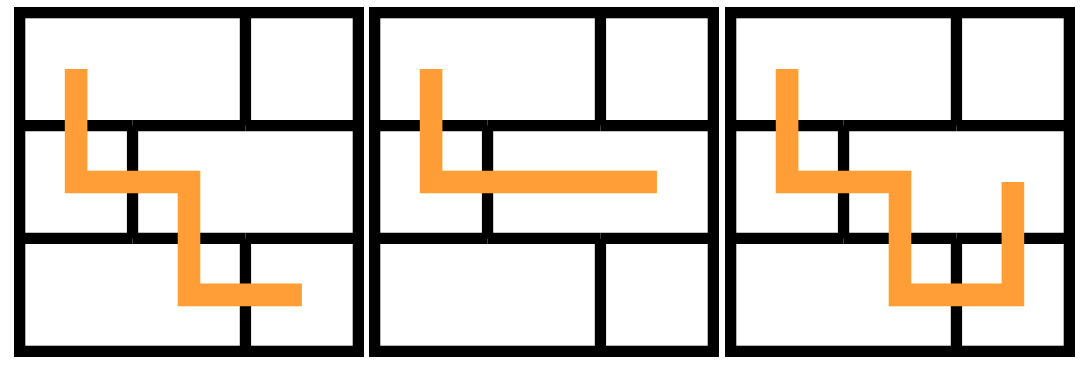
\includegraphics[width=0.7\linewidth]{path.png}
    \caption{以上三個圖中,只有最左邊的路徑滿足以上條件。中間的路徑,同一個磁磚被連續走過兩次。在右邊的路徑,他在離開磁磚後,又回到了同一塊磁磚。}
\end{figure}

\begin{figure}[H]
    \centering
    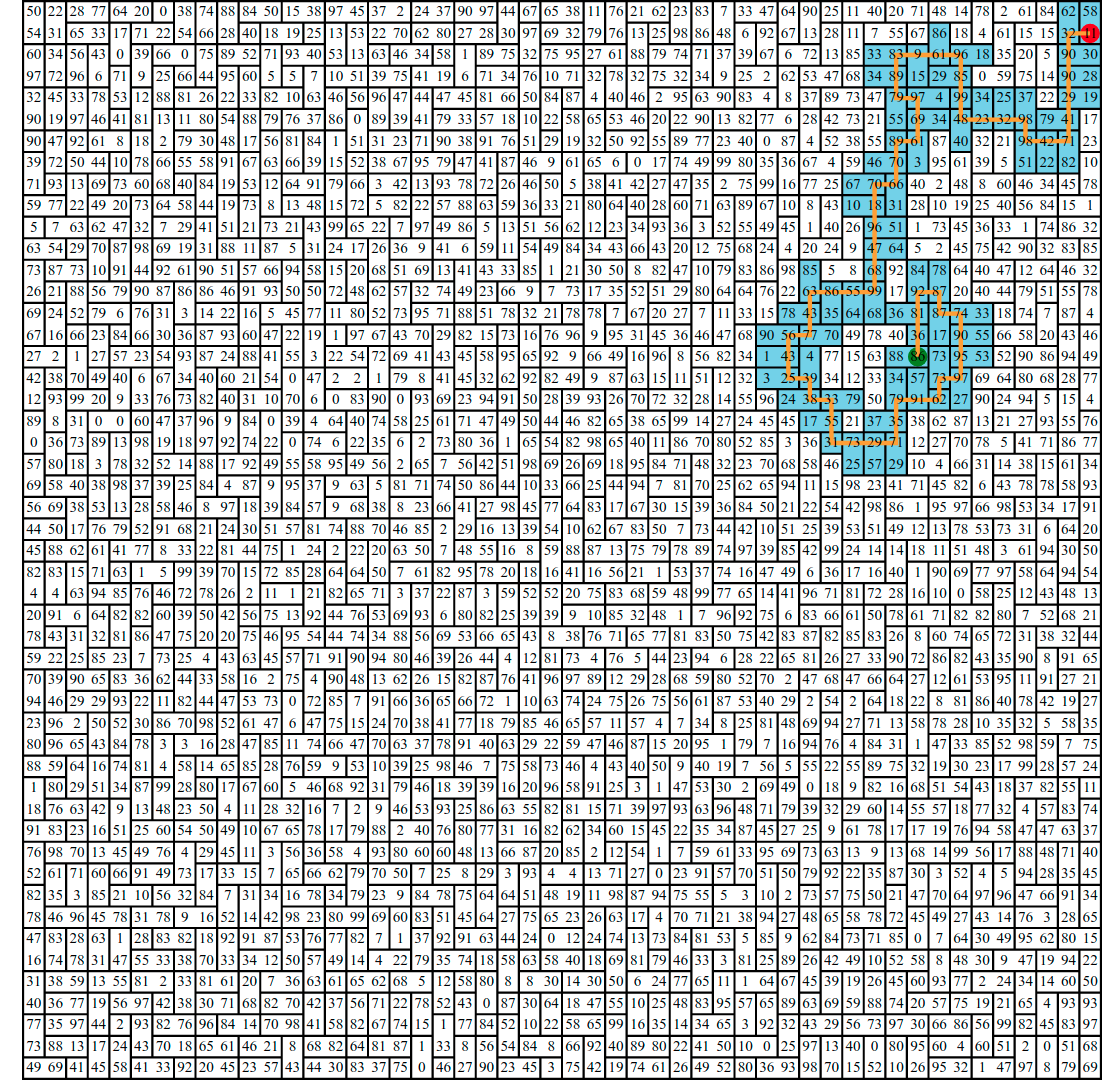
\includegraphics[width=0.7\linewidth]{map.png}
    \caption{範例測試資料中的其中一條合法路徑 (但顯然不是最佳路徑)。紅色圈圈代表初始位置,綠色圈圈代表最終位置。走過的磁磚以淺藍色表示。}
\end{figure}

\subsection{程式輸入}

\begin{array}{lllc}
s_i & s_j\\
t_{0,0} & t_{0,1} & \ldots & t_{0,49} \\
\vdots & & & \\
t_{49,0} & t_{49,1} & \ldots & t_{49,49} \\
p_{0,0} & p_{0,1} & \ldots & p_{0,49} \\
\vdots & & & \\
p_{49,0} & p_{49,1} & \ldots & p_{49,49}
\end{array}

\begin{itemize}
    \item $(s_i, s_j)$代表初始位置且滿足$0 \leq s_i, s_j \leq 49$。
    \item $t_{i, j}$ 是一個整數,代表在$(i, j)$的磁磚。如果$t_{i, j} = t_{i', j'}$,則$(i, j), (i', j')$屬於同一個磁磚。
    \item $p_{i, j}$是一個整數,滿足$0 \leq p_{i, j} \leq 49$,代表$(i, j)$的分數。
\end{itemize}

\subsection{程式輸出}
以\texttt{U, D, L, R}分別表示從$(i, j)$到$(i-1, j), (i+1, j), (i, j-1), (i, j+ 1)$。並輸出一個字串表示路徑。

\subsection{時間及記憶體限制}
\begin{itemize}
    \item 時間限制: 2 秒
    \item 記憶體限制: 1024 MB
\end{itemize}
\section{研究目的}

找到一個能在兩秒內找出使路徑分數盡可能高的演算法。

\section{研究過程與方法}
\subsection{基礎演算法介紹}
\subsubsection{深度優先搜尋 (Depth-First Search; DFS)}
深度優先搜尋是一種用於遍歷圖或樹的演算法。這種演算法會盡可能深的搜尋樹的分支。若所有分支皆已遍歷,則會回朔到起始節點。

\begin{figure}[H]
    \centering
    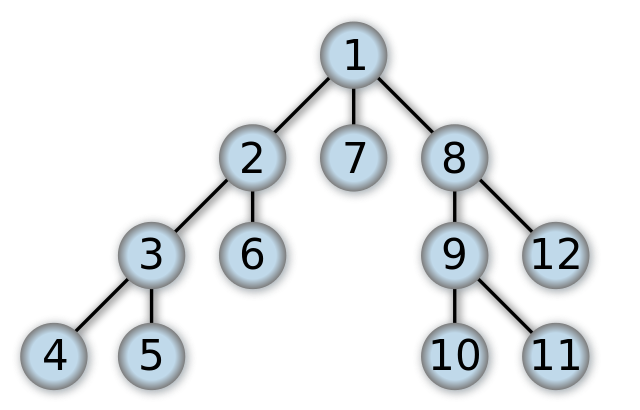
\includegraphics[width=0.7\linewidth]{dfs.png}
    \caption{以DFS遍歷此顆樹的結果,節點中的數字代表遍歷到的順序。\\ (取自: 維基百科 - 深度優先搜尋)}
\end{figure}

實務上,我們會使用遞迴(recursion)的方式來實作DFS演算法,具體方式如下:

\begin{code}
\captionof{listing}{DFS在C++的實作 (使用相鄰串列)}
\begin{minted}
#include <bits/stdc++.h>
using namespace std;
const int N = 10;

vector<vector<int>> adj(N);
vector<bool> vis(N, false);

void dfs(int source){
    vis[source] = true;
    cout << source << endl;
    
    for(auto i: adj[source])     
        if(vis[i] == false) dfs(i);
}

int main(){
    dfs(0);
}
\end{minted}
\end{code}

DFS演算法的時間複雜度為$O(b^m)$,其中$b$為分支因子 (branching factor),$m$為遞迴深度。

% \subsubsection{模擬退火 (Simulated annealing; SA)}

\subsection{測試資料及演算法評分}

本研究使用AtCoder網站所提供的測試資料,共有100筆,皆為隨機生成。

在測試演算法時,我們將100筆測試資料輸入到程式中,並將100筆的路徑分數加總,成為該演算法的總分。

測試資料可以在\url{https://github.com/jayin92/walking-on-tiles/testcase/}中 \\ 找到。

\subsection{本研究之演算法}
本研究主要討論三種演算法,分別為純DFS、優先往最近邊界方向的DFS及隨機方向的DFS。

前述提到DFS的時間複雜度為$O(b^m)$,而在Walking On Tiles中,最壞情況時,$b=4, m=50\times50=2500$,故最差時間複雜度為$O(4^{2500}) \approx O(1.41 \times 10^{1505})$。在最壞情況下,不可能在兩秒內找出最佳解,故本研究的程式會紀錄目前找到的最佳解,並在接近兩秒時中止遞迴並輸出目前找到的最佳答案。

\subsubsection{純DFS}

純DFS的方式是對於每一個方塊,檢查與其相鄰的四個方塊是否違反路徑規則,若無則繼續往下遞迴。其片段程式碼如下:

\begin{code}
\captionof{listing}{純DFS}
\begin{minted}
#include <bits/stdc++.h>

using namespace std;
typedef long long ll;
typedef pair<int, int> pii;

const int N = 50;

pii d[4] = {{1, 0}, {-1, 0}, {0, 1}, {0, -1}};
char con[4] = {'D', 'U', 'R', 'L'};
vector<int> order = {0, 1, 2, 3};


inline bool check(pii nxt, vector<bool> vis){
    if(nxt.X >= N || nxt.Y >= N || nxt.X < 0 || nxt.Y < 0) return false;
    if(vis[ti[nxt.X][nxt.Y]] == true) return false;
 
    return true;
}

inline pii add(pii a, pii b){
    return make_pair(a.X + b.X, a.Y + b.Y);
}

void walk(pii s, vector<bool> vis, ll score, string path){
    vis[ti[s.X][s.Y]] = true;
    score += sc[s.X][s.Y];
    bool flag = true;
    int i;
    for(int j=0;j<4;j++){
        i = order[j];
        pii nxt = add(s, d[i]);
        if(check(nxt, vis)){
            flag = false;
            walk(nxt, vis, score, path+con[i]);           
        }
    }
    if(flag){
        if(score > max_score){
            max_score = score;
            ans = path;
        }
    }
}
\end{minted}
\end{code}

由於DFS的性質,我們可以發現有關遍歷方向順序的\texttt{vector<int> order}陣列對於路徑的搜尋至關重要。故在本研究中,我們測試了全部$4!=24$組合,並探討其對於路徑總分的影響。

\subsubsection{隨機方向的DFS}

本方法則是從24種方向順序中,選出其中一種當作目前這步的方向順序,具體程式碼如下:

\begin{code}
\captionof{listing}{隨機方向的DFS}
\begin{minted}
#include <bits/stdc++.h>

using namespace std;
typedef long long ll;
typedef pair<int, int> pii;

const int N = 50;

pii d[4] = {{1, 0}, {-1, 0}, {0, 1}, {0, -1}};
char con[4] = {'D', 'U', 'R', 'L'};
vector<int> order = {0, 1, 2, 3};


inline bool check(pii nxt, vector<bool> vis){
    if(nxt.X >= N || nxt.Y >= N || nxt.X < 0 || nxt.Y < 0) return false;
    if(vis[ti[nxt.X][nxt.Y]] == true) return false;
 
    return true;
}

inline pii add(pii a, pii b){
    return make_pair(a.X + b.X, a.Y + b.Y);
}

void walk(pii s, vector<bool> vis, ll score, string path){
    vis[ti[s.X][s.Y]] = true;
    score += sc[s.X][s.Y];
    bool flag = true;
    int i;
    random_shuffle(order.begin(), order.end());
    for(int j=0;j<4;j++){
        i = order[j];
        pii nxt = add(s, d[i]);
        if(check(nxt, vis)){
            flag = false;
            walk(nxt, vis, score, path+con[i]);           
        }
    }
    if(flag){
        if(score > max_score){
            max_score = score;
            ans = path;
        }
    }
}
\end{minted}
\end{code}


\subsubsection{優先往最近邊界方向的DFS}

由於同一片磁磚只能走過一次,使用隨機方向可能會使大部分方塊無法被走過。於是我就設想若能使 Takahashi 盡量貼著邊界走,並逐漸往中間繞,是否就可以讓大部分方塊能被探訪,並使路徑分數提高。

我將$50 \times 50$的方塊分成四個部份,分別為$(0, 0), (24, 2 4)$、$(25, 0), (49, 24)$、\\ $(0, 25), (24, 49)$及$(25, 25), (49, 49)$ ($(a, b)$ $a$為左上邊界,$b$為右下邊界),對於每個部份再判定往哪個方向前進能最快到達邊界。具體程式碼如下:
\begin{code}
\captionof{listing}{純DFS}
\begin{minted}
#include <bits/stdc++.h>

using namespace std;
typedef long long ll;
typedef pair<int, int> pii;

const int N = 50;

pii d[4] = {{1, 0}, {-1, 0}, {0, 1}, {0, -1}};
char con[4] = {'D', 'U', 'R', 'L'};
vector<int> order = {0, 1, 2, 3};


inline bool check(pii nxt, vector<bool> vis){
    if(nxt.X >= N || nxt.Y >= N || nxt.X < 0 || nxt.Y < 0) return false;
    if(vis[ti[nxt.X][nxt.Y]] == true) return false;
 
    return true;
}

inline pii add(pii a, pii b){
    return make_pair(a.X + b.X, a.Y + b.Y);
}

void walk(pii s, vector<bool> vis, ll score, string path){
    vis[ti[s.X][s.Y]] = true;
    score += sc[s.X][s.Y];
    bool flag = true;
    pii nxt = add(s, d[dir]);

    int i;
    vector<int> dis(4);
    // D U R L
    if(s.X <= 24){
        if(s.Y <= 24){
            if(s.X < s.Y){
                dis = {1, 3, 2, 0};
            } else {
                dis = {3, 1, 0, 2};
            }
        } else {
            if(s.X < abs(49 - s.Y)){
                dis = {1, 2, 3, 0};
            } else {
                dis = {2, 1, 0, 3};
            }         
        }
    } else {
        if(s.Y <= 24){
            if(abs(49 - s.X) < s.Y){
                dis = {0, 3, 2, 1};
            } else {
                dis = {3, 0, 1, 2};
            }
        } else {
            if(abs(49 - s.X) < abs(49 - s.Y)){
                dis = {0, 2, 3, 1};
            } else {
                dis = {2, 0, 1, 3};
            }
        }
    }

    for(int j=0;j<4;j++){
        i = dis[j];
        nxt = add(s, d[i]);
        if(check(nxt, vis)){
            flag = false;
            walk(nxt, vis, score, path+con[i], i);           
        }
    }
 
    if(flag){
        cnt ++;
        if(score > max_score){
            max_score = score;
            ans = path;
        }
    }
 
    return;
}
\end{minted}
\end{code}

\subsection{演算法測試方式}
\subsubsection{純DFS}
在純DFS的測試中,需要將24種方向順序分別執行和計算路徑總分,故本研究額外在編寫了一簡單的Python程式,其可以執行編譯後的C++程式並紀錄結果。而窮舉24種組合的方式則是使用Python內建的\texttt{itertools.permutation()}。具體Python程式碼如下:
\begin{code}
\captionof{listing}{測試用 Python 程式碼 (純DFS)}
\begin{mintedPython}
import subprocess
import tqdm
import itertools
import statistics

total_score = 0

order = [0, 1, 2, 3];
for item in itertools.permutations(order):
    total_score = 0
    test_res = []
    for i in tqdm.tqdm(range(100)):
        file_path = "testcase/" + '0' * (4 - len(str(i))) + str(i) + '.txt';
        com = "./solve.out {} {} {} {} < {}".format(item[0], item[1], item[2], item[3], file_path)

        sub_pro = subprocess.Popen(com, shell=True, stdout=subprocess.PIPE);
        
        out = int(sub_pro.stdout.read())
        print(out)
        total_score += out
        test_res.append(out)

    res = "{} Score: {}, STD: {}, {}".format(item, total_score, statistics.stdev(test_res), test_res)
    print(res)
    with open("results.txt", "a") as file:
        file.write(res+"\n")
\end{mintedPython}
\end{code}
\subsubsection{隨機方向及優先往最近邊界方向DFS}
因為這兩種演算法不需要額外輸入方向順序的參數,故測試用Python程式碼較為簡單,具體如下:

\begin{code}
\captionof{listing}{測試用 Python 程式碼 (隨機方向及優先往最近邊界方向DFS)}
\begin{mintedPython}
import subprocess
import tqdm
import itertools
import statistics

total_score = 0

order = [0, 1, 2, 3]

test_res = []
for i in tqdm.tqdm(range(100)):
    file_path = "testcase/" + '0' * (4 - len(str(i))) + str(i) + '.txt';
    com = "./solve_wfs.out < {}".format(file_path)

    sub_pro = subprocess.Popen(com, shell=True, stdout=subprocess.PIPE);
    
    out = int(sub_pro.stdout.read())
    print(out)
    total_score += out
    test_res.append(out)

res = "Score: {}, STD: {}, {}".format(total_score, statistics.stdev(test_res), test_res)

print(res)
\end{mintedPython}
\end{code}

\section{研究結果}
\subsection{三種演算法的測試結果}
\subsubsection{純DFS}
\begin{table}[H]
\caption{不同方向順序的純DFS的100筆測資總分及其標準差}
\label{tab:my-table}
\centering
\begin{tabular}{@{}ccc@{}}
\toprule
\textbf{order} & \textbf{總分} & \textbf{標準差} \\ \midrule
(0, 1, 2, 3)   & 2670985     & 10463.27     \\
(0, 1, 3, 2)   & 2731881     & 9378.54      \\
(0, 2, 1, 3)   & 3522972     & 10664.87     \\
(0, 2, 3, 1)   & 3916793     & 9902.49      \\
(0, 3, 1, 2)   & 3545963     & 9312.88      \\
(0, 3, 2, 1)   & 3796590     & 10440.81     \\
(1, 0, 2, 3)   & 2921168     & 9667.44      \\
(1, 0, 3, 2)   & 3026720     & 8825.52      \\
(1, 2, 0, 3)   & 3794062     & 8149.56      \\
(1, 2, 3, 0)   & 4040987     & 9077.79      \\
(1, 3, 0, 2)   & 3782214     & 8248.43      \\
\textbf{(1, 3, 2, 0)}   & \textbf{4097473}     & \textbf{8213.99}      \\
(2, 0, 1, 3)   & 3965513     & 9481.04      \\
(2, 0, 3, 1)   & 3699186     & 9307.27      \\
(2, 1, 0, 3)   & 4031891     & 9081.29      \\
(2, 1, 3, 0)   & 3676140     & 9796.02      \\
(2, 3, 0, 1)   & 2738225     & 9739.35      \\
(2, 3, 1, 0)   & 2929852     & 9758.51      \\
(3, 0, 1, 2)   & 3981065     & 8248.62      \\
(3, 0, 2, 1)   & 3897014     & 7313.75      \\
(3, 1, 0, 2)   & 4091678     & 8975.19      \\
(3, 1, 2, 0)   & 3703809     & 9159.63      \\
(3, 2, 0, 1)   & 2974666     & 7738.07      \\
(3, 2, 1, 0)   & 2742744     & 10369.69     \\ \bottomrule
\end{tabular}
\end{table}

由上表可以發現,不同方向順序間的總分差距十分明顯,且由測試可知最佳的方向順序為$(1, 3, 2, 0)$ (即為 \texttt{(U, L, R, D)}),在100筆測試資料中,取得了總分4097473的分數,且標準差相較於其他方向並沒有顯著的差距。

\subsubsection{隨機方向的DFS}
\begin{table}[H]
\caption{不同方向順序的純DFS的100筆測資總分及其標準差}
\label{tab:my-table}
\centering
\begin{tabular}{@{}ccc@{}}
\toprule
\textbf{總分} & \textbf{標準差} \\ \midrule
1843341     & 7872.47    \\
 \bottomrule
\end{tabular}
\end{table}

可以發現使用隨機方式的總分相較於固定方向順序是相當的低,我猜測是因為使用隨機方式會使大部分方塊無法被探訪到。
\subsubsection{優先往邊界方向的DFS}
\begin{table}[H]
\caption{優先往邊界方向的DFS的100筆測資總分及其標準差}
\label{tab:my-table}
\centering
\begin{tabular}{@{}ccc@{}}
\toprule
\textbf{總分} & \textbf{標準差} \\ \midrule
4421451     & 7124.66      \\
\bottomrule
\end{tabular}
\end{table}

可以發現使用優先往邊界方向的DFS會使總分最高,由下節的路徑圖可以發現這是因為其會盡量貼著邊界走,使未走過的磁磚數降到最低。

\subsection{三種演算法的路徑}
在本節中,我們將第一筆測試資料輸入到三種演算法中,其中純DFS使用效果最好的(1, 3, 2, 0)順序。

\begin{figure}[H]
    \centering
    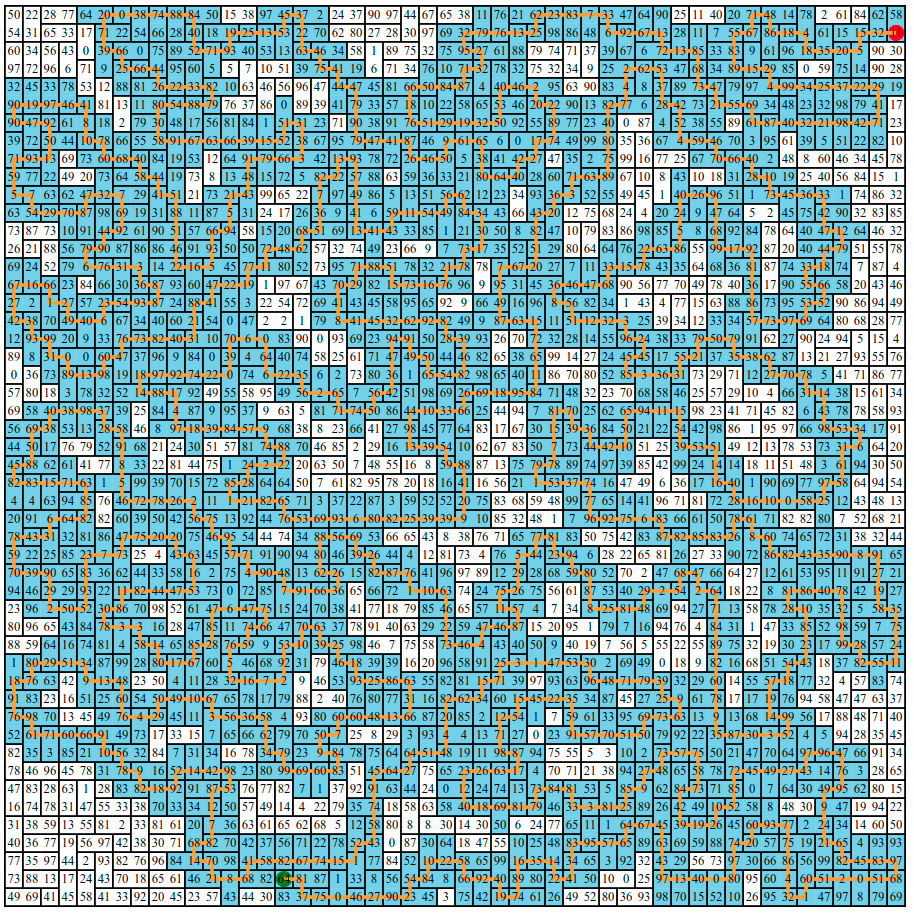
\includegraphics[width=0.6\linewidth]{path_dfs.png}
    \caption{純DFS的路徑 (使用(1, 3, 2, 0)順序)}
\end{figure}

\begin{figure}[H]
    \centering
    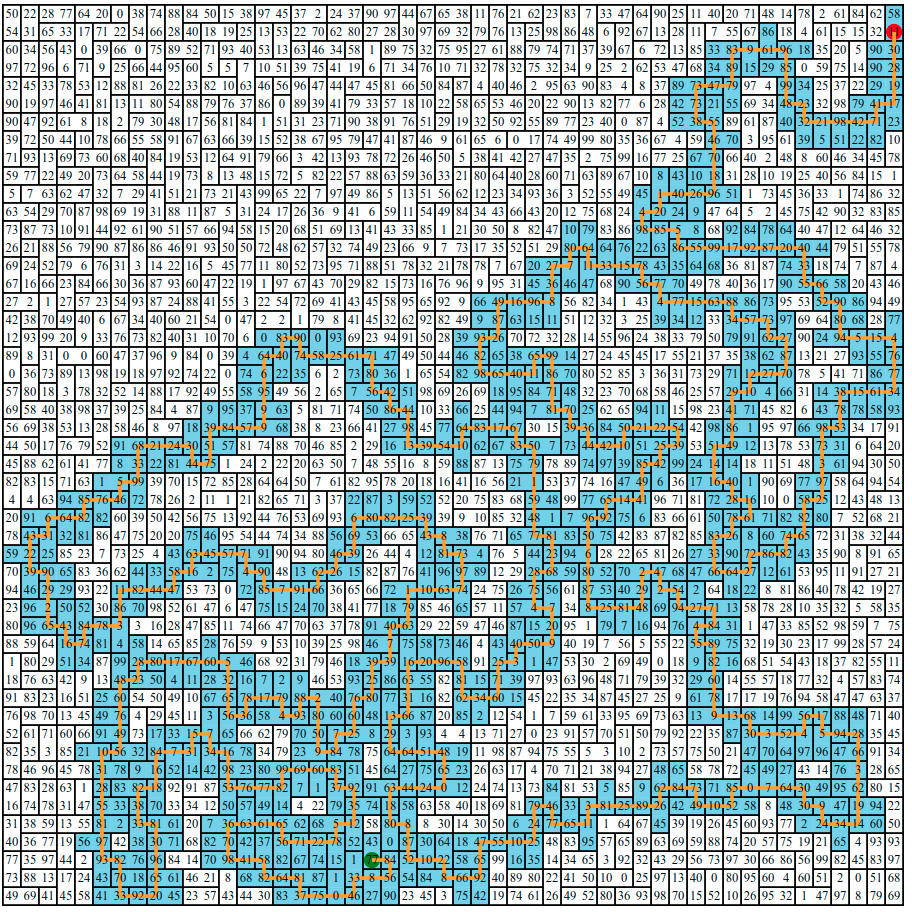
\includegraphics[width=0.6\linewidth]{path_ran.png}
    \caption{隨機方向DFS的路徑}
\end{figure}

\begin{figure}[H]
    \centering
    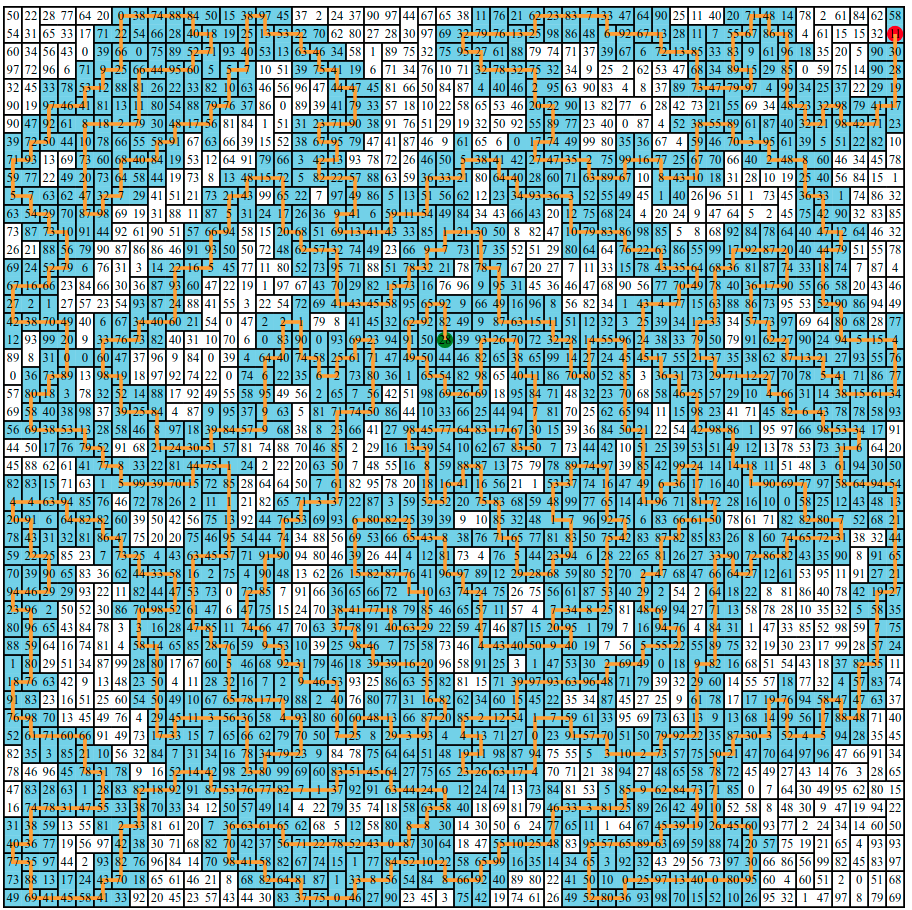
\includegraphics[width=0.6\linewidth]{path_wfs.png}
    \caption{優先往邊界方向的DFS}
\end{figure}

\section{結論與未來展望}
\subsection{結論}

由以上研究我們可以知道,對於純DFS來說,使用方向順序(1, 3, 2, 0)會使結果最好。整體而言,使用優先往最近邊界的方式會使結果最佳,純DFS其次,最差的則為隨機方向DFS。

\subsection{未來展望}

本題若使用模擬退火法 (Simulated Annealing; SA)會使路徑總分達到約600萬分。但由於筆者能力不足,對於模擬退火法沒有很深的認識,期望未來可以分析在本題使用模擬退火法的效果。

\nocite{*}
\printbibliography[title={參考文獻}]

\end{document}
